\subsection{三角形三边的关系}\label{subsec:czjh1-3-2}

\begin{wrapfigure}[8]{r}{5cm}
    \centering
    \begin{tikzpicture}
    \tkzDefPoints{0/0/B, 3.5/0/C, 2.8/2/A}

    \tkzDrawPolygon(A,B,C)
    \tkzLabelSegment[below](B,C){$a$}
    \tkzLabelSegment[above right](A,C){$b$}
    \tkzLabelSegment[above left](A,B){$c$}
    \tkzLabelPoints[above](A)
    \tkzLabelPoints[left](B)
    \tkzLabelPoints[right](C)
\end{tikzpicture}


    \caption{}\label{fig:czjh1-3-7}
\end{wrapfigure}


在 $\triangle ABC$ 中,$\angle A$、$\angle B$、$\angle C$ 所对的边 $BC$、$CA$、$AB$,
通常用 $a$、$b$、$c$ 表示(图 \ref{fig:czjh1-3-7})。 我们知道,两点间线段最短。根据这个公理,得

$b + c > a$, $c + a > b$, $a + b > c$。

由此得到:

\begin{dingli}[定理]
    三角形任何两边的和大于第三边。
\end{dingli}

从定理直接推出来的定理叫做\zhongdian{推论}。从上述的定理可以得出如下的推论:

\begin{tuilun}[推论]
    三角形任何两边的差小于第三边。
\end{tuilun}

例如,如果 $a \geqslant b$, 那么, 从 $b + c > a$, 可以推出 $c > a - b$,(为什么?) 即 $a - b < c$。

有的三角形,三条边各不相等,有的有两条边相等,有的三条边都相等。
因此,三角形可以按照边进行分类。

三边两两不等的三角形叫做\zhongdian{不等边三角形}(图 \ref{fig:czjh1-3-8} 甲)。
三边中有两边相等的三角形叫做\zhongdian{等腰三角形}(图 \ref{fig:czjh1-3-8} 乙)。
三边都相等的三角形叫做\zhongdian{等边三角形}(图 \ref{fig:czjh1-3-8} 丙)。

\begin{figure}[htbp]
    \centering
    \begin{minipage}[b]{4.5cm}
        \centering
        \input{../pic/czjh1-ch3-08-a}
        \caption*{甲}
    \end{minipage}
    \qquad
    \begin{minipage}[b]{4cm}
        \centering
        \begin{tikzpicture}
    \tkzDefPoints{0/0/B, 2.6/0/C, 1.3/3/A}

    \tkzDrawPolygon(A,B,C)
    \tkzMarkSegments[mark=||](A,B  A,C)
    \tkzLabelPoints[above](A)
    \tkzLabelPoints[below](B,C)
\end{tikzpicture}


        \caption*{乙}
    \end{minipage}
    \begin{minipage}[b]{4cm}
        \centering
        \begin{tikzpicture}
    \tkzDefPoints{0/0/B, 3/0/C}
    \tkzDefTriangle[equilateral](B,C)  \tkzGetPoint{A}

    \tkzDrawPolygon(A,B,C)
    \tkzMarkSegments[mark=|](A,B  A,C  B,C)
    \tkzLabelPoints[above](A)
    \tkzLabelPoints[below](B,C)
\end{tikzpicture}


        \caption*{丙}
    \end{minipage}
    \caption{}\label{fig:czjh1-3-8}
\end{figure}

在等腰三角形中,相等的两边都叫做\zhongdian{腰},另外一边叫做\zhongdian{底边},
两腰的夹角叫做\zhongdian{顶角}, 腰和底边的夹角叫做\zhongdian{底角}。

等边三角形是特殊的等腰三角形,即底边和腰相等的等腰三角形。

三角形集合包含不等边三角形集合和等腰三角形集合,
而等腰三角形集合,又包含底边和腰不相等的等腰三角形集合和等边三角形集合。


$$
    \text{三角形} \smash[t]{\left\{ \begin{aligned}
        &\text{不等边三角形} \\[1.5em]
        & \text{等腰三角形} \smash{\left\{ \begin{aligned}
            &\text{底边和腰不相等的等腰三角形} \\
            &\text{等边三角形}
        \end{aligned} \right.}
    \end{aligned} \right.}
$$ \vspace*{.5em}


\liti[0] 已知:在 $\triangle ABC$ 中, $D$ 是边 $AB$ 上任意一点(图 \ref{fig:czjh1-3-9} )。

求证: $AB + AC > DB + DC$。

\zhengming 在 $\triangle ADC$ 中,

$\because$ \quad $AD + AC > DC$ (三角形两边的和大于第三边),

$\therefore$ \quad $AD + DB + AC > DB + DC$ (不等式的性质),

即 \hspace*{3.2em} $AB + AC > DB + DC$。

\begin{figure}[htbp]
    \centering
    \begin{minipage}[b]{7cm}
        \centering
        \begin{tikzpicture}
    \tkzDefPoints{0/0/B, 3.5/0/C, 2.2/2/A}
    \tkzDefPointOnLine[pos=0.2](A,B)  \tkzGetPoint{D}

    \tkzDrawPolygon(A,B,C)
    \tkzDrawSegments(C,D)
    \tkzLabelPoints[above](A)
    \tkzLabelPoints[left](B)
    \tkzLabelPoints[above, xshift=-0.3em](D)
    \tkzLabelPoints[right](C)
\end{tikzpicture}


        \caption{}\label{fig:czjh1-3-9}
    \end{minipage}
    \qquad
    \begin{minipage}[b]{7cm}
        \centering
        % 满足题设的三角形,角 A = 36度, 角 B = 角 C = 72度。
\begin{tikzpicture}
    \pgfmathsetmacro{\bc}{2}
    \tkzDefPoints{0/0/B, \bc/0/C}
    \tkzDefPointBy[rotation=center B angle  72](C)  \tkzGetPoint{a1}
    \tkzDefPointBy[rotation=center C angle -72](B)  \tkzGetPoint{a2}
    \tkzInterLL(B,a1)(C,a2)  \tkzGetPoint{A}
    \tkzInterCC[R](A,\bc)(B,\bc)  \tkzGetFirstPoint{D}

    \tkzDrawPolygon(A,B,C)
    \tkzDrawSegments(B,D)
    \tkzLabelPoints[above](A)
    \tkzLabelPoints[left](B)
    \tkzLabelPoints[right](C,D)
\end{tikzpicture}


        \caption*{(第 2 题)}
    \end{minipage}
\end{figure}

\begin{lianxi}

\xiaoti{(口答)有下列长度的三条线段能否组成三角形?为什么?}
\begin{xiaoxiaotis}

    \begin{tblr}{colsep=0pt}
        \xxt{3 cm,4 cm,8 cm;}
            & \xxt{5 cm,6 cm,11 cm;}
            & \xxt{5 cm,6 cm,10 cm;}
    \end{tblr}

\end{xiaoxiaotis}


\xiaoti{(口答) 如图,已知点 $D$ 在 $AC$ 上, $AB = AC$, $AD = BD = BC$。
    图中有几个等腰三角形? 是哪几个? 说出它们的腰、底边、顶角和底角。
}

\xiaoti{以 4 cm 长的线段为底,1 cm 长的线段为腰,能否组成一个等腰三角形?
    如果以 4 cm 长为底组成一个等腰三角形,腰长应在什么范围内?
}

\end{lianxi}

